\subsection*{Item c}
\addcontentsline{toc}{subsection}{Item c}

\begin{lstlisting}[language=Python]
parameter_interval = np.array(range(2, 50, 5))
image = mpimg.imread("data/araras.png")

# Geracao das imagens comprimidas
for i in parameter_interval:
    tmp = function_1(image, i)
    plt.imsave(f"../results/imagem_{i}.png", tmp)

# Calculo das taxas de compressao
original_size = os.path.getsize("data/araras.png")
sizes = []
for i in parameter_interval:
    file_size = os.path.getsize(f"../results/imagem_{i}.png")
    sizes.append(file_size / original_size)

theoretical_sizes = np.ceil(np.log2(parameter_interval)) / 24

# Plotagem das curvas real vs teorica
\end{lstlisting}

\begin{figure}[H]
    \centering
    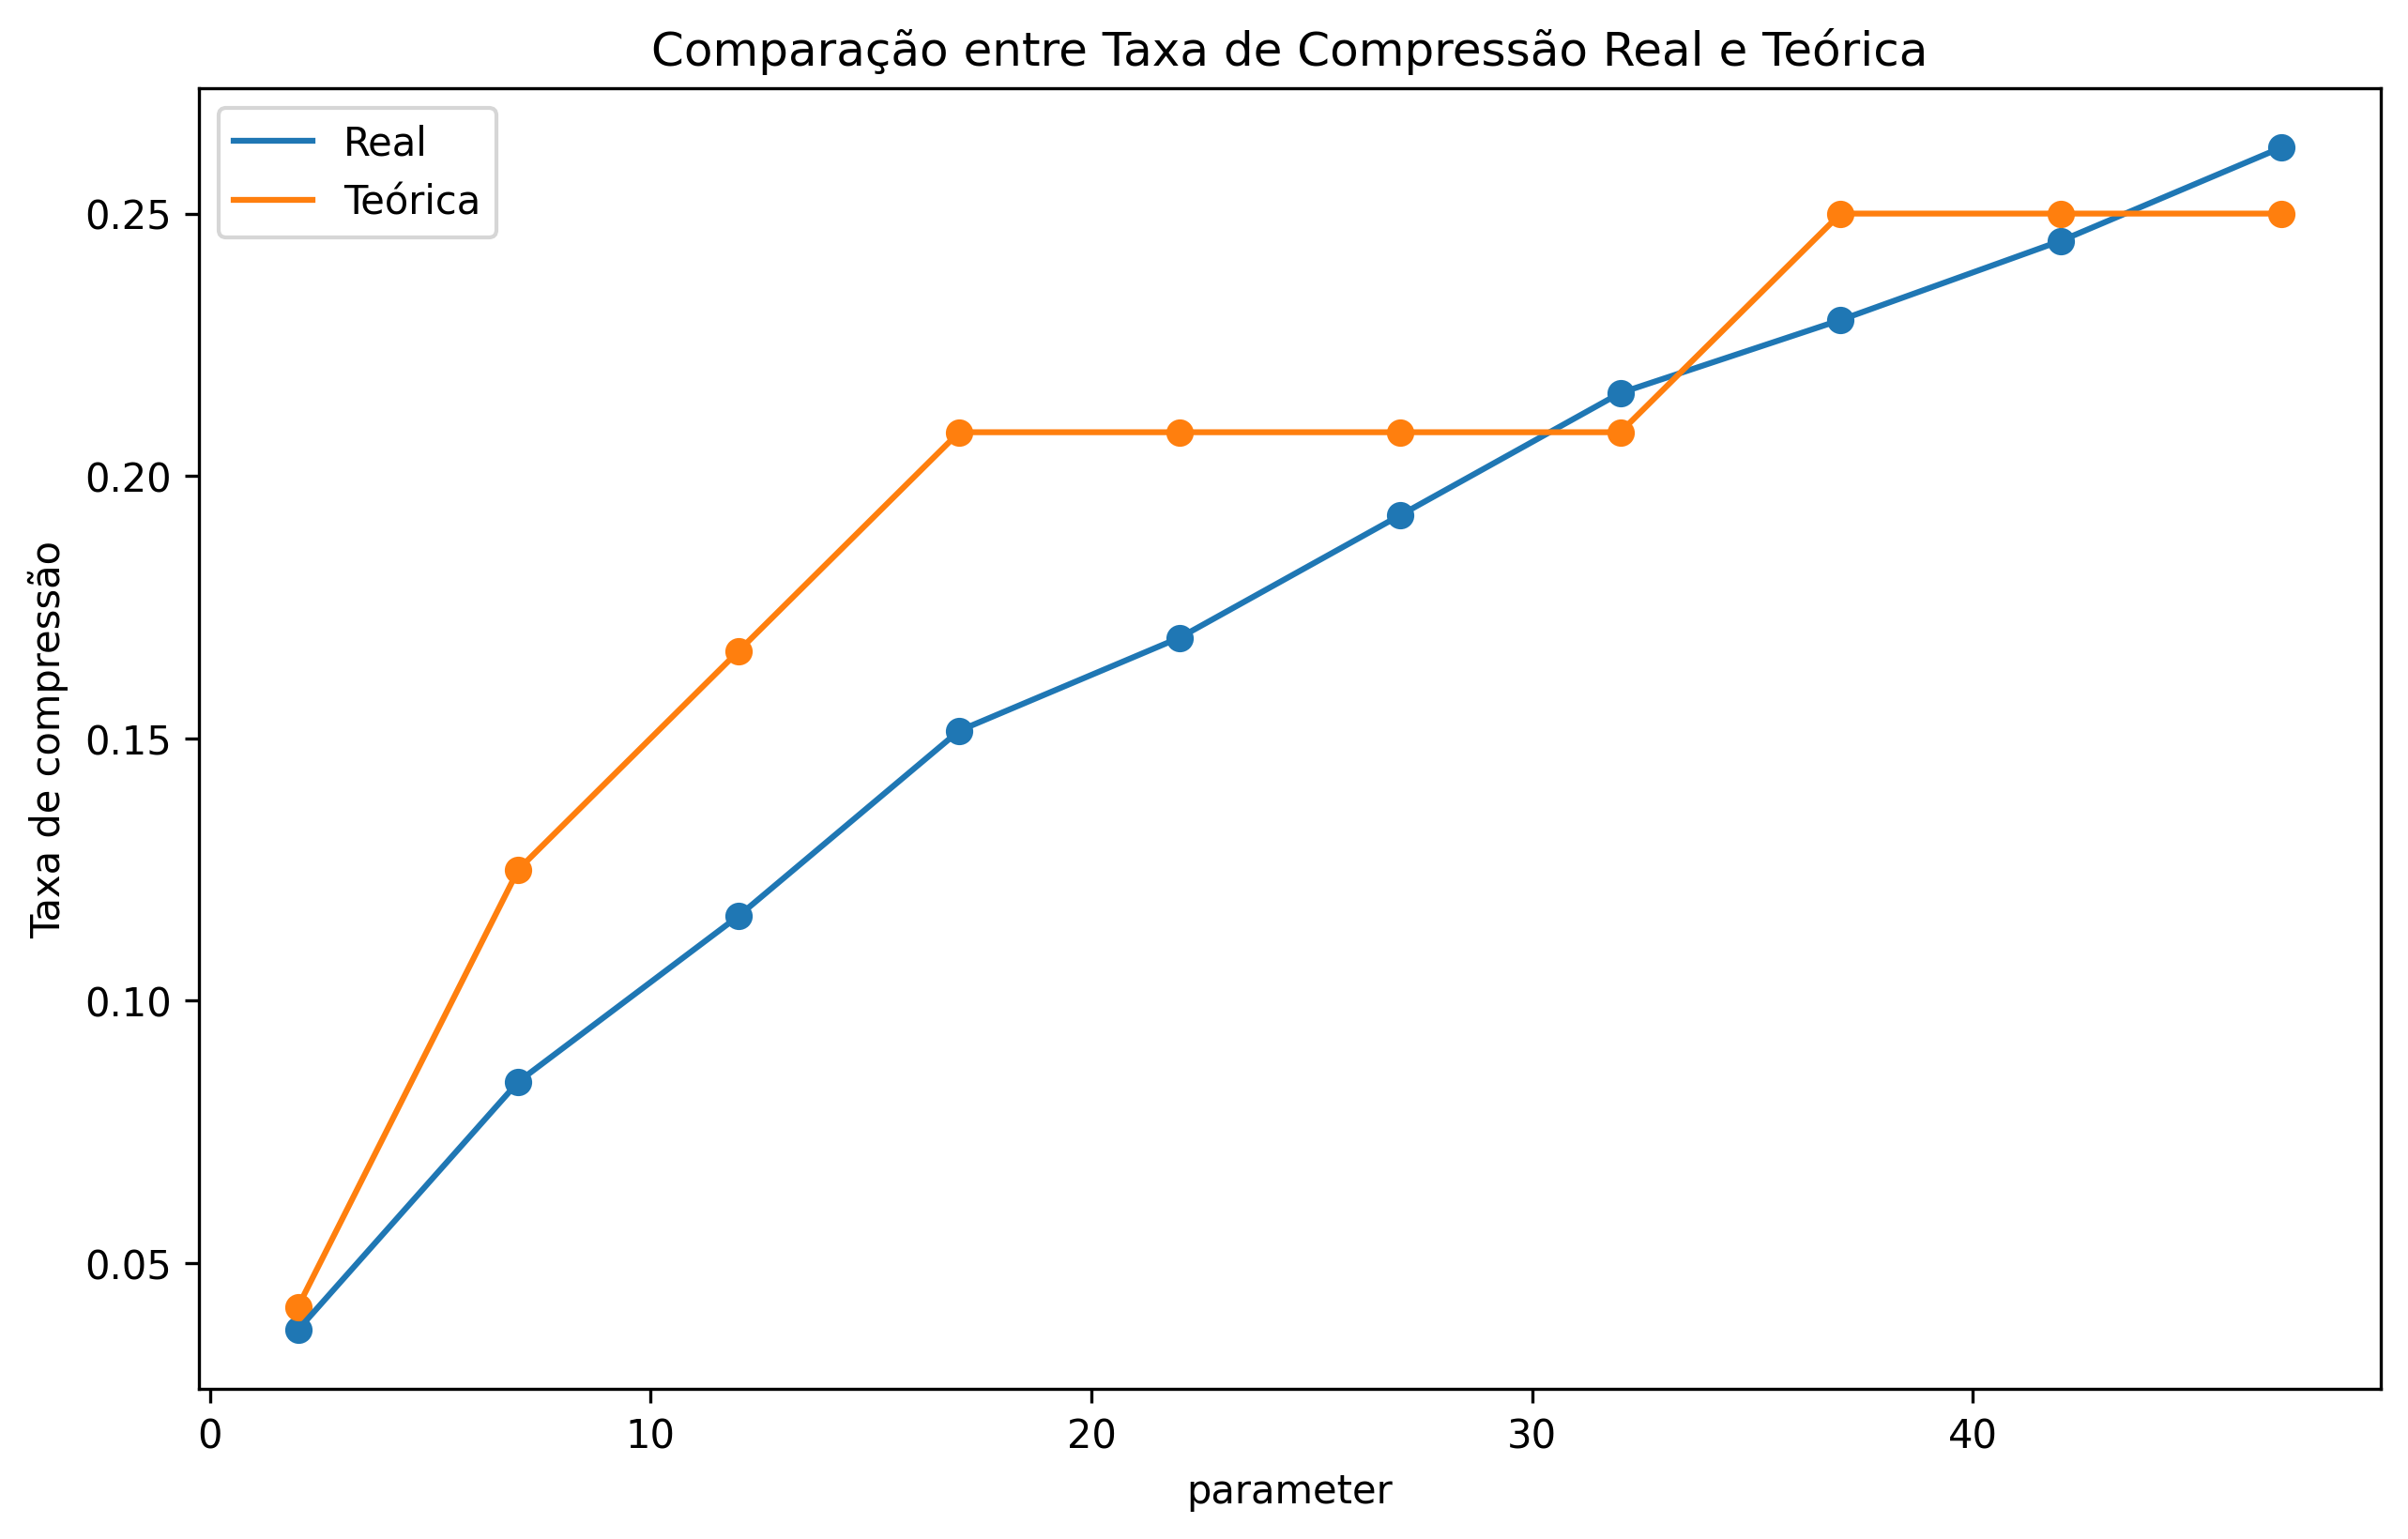
\includegraphics[width=0.8\textwidth]{../figures/5/compression_rates.png}
    \caption{Comparação entre taxa de compressão real e teórica}
    \label{fig:compression_rates}
\end{figure}


A taxa de compressão verificada é calculada considerando o arquivo em toda a sua extensão, o que inclui seus metadados, headers e técnicas de compressão do formato PNG.
Em contrapartida, os valores teóricos consideravam apenas a equivalência bit a bit, não considerando a matriz com o armazenamento das classes. Caso fosse considerada,
ela adicionaria um termo $\frac{\text{parameter}}{\text{num\_pixels}}$ ao valor teórico da taxa de compressão, o que, para o caso desta imagem, seria próximo a 0.

Assim, a taxa de compressão real foi menor do que a taxa teórica para valores baixos de parameter, o que pode ser explicado pelas técnicas de compressão
adotadas pelo formato PNG, que são mais eficientes para imagens com menos variação de cores e a menor quantidade de headers.

À medida que o número de clusters aumenta, a taxa de compressão verificada se aproxima da taxa teórica, até que esta torna-se mais eficiente para valores mais
altos de parameter. Isso pode ser explicado pela presença de maior quantidade de metadados e menor eficiência das técnicas de compressão do formato PNG para
imagens com maior variação de cores.